% Roll no 55, Sayooj Surendran
\textbf{\textcolor{LightMagenta}{Calculate the output y of a three input neuron with bias. The input feature vector is (x1, x2,x3)= (0.8,0.6,0.4) and weight values are [w1,w2,w3, b]  [0.2, 0.1, -0.3, 0.35]. Use binary Sigmoid function as activation function. (Sept 2020) \hfill 4 marks}} \\[5pt]

An artificial neuron is a mathematical function conceived as a model of biological
neurons. Artificial neurons are elementary units in an artificial neural network. The
artificial neuron receives one or more inputs and sums them to
produce an output. Each input is separately weighted, and the sum is passed through a
function known as an activation function or transfer function. \\[5pt]
The output y of a neural network is given by f($\sum_{i=1}^n w_ix_i$+b) . Where f is the activation function. For binary Sigmoid function as activation function,\\ 

f(x) = \begin{math} ( \frac{1}{ 1+ e^{-x} }  \end{math}
\begin{center}
  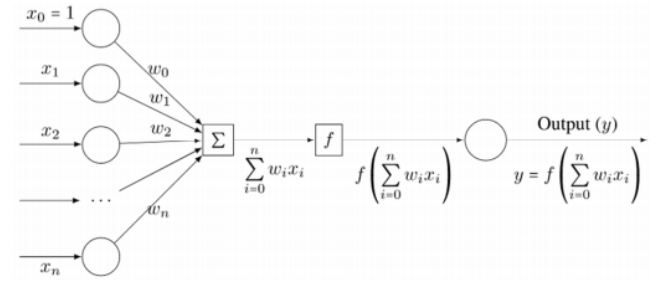
\includegraphics[width=.8\textwidth]{Images/A18_IMG1.png}  
\end{center}

\textcolor{purple}{\underline{Answer}} \\
First we calculate sum \begin{math} \Sigma_{n=1}^3 w_ix_i \\ [5pt]
\Sigma_{n=1}^3 w_ix_i +b  = 0.8*0.2 + 0.6*0.1 + 0.4*(-0.3) + 0.35 = 0.45
\\ [5pt]
Output y = f(sum_{i=1}^3 w_ix_i+b) \\ [5pt]
\end{math}
Where f is binary Sigmoid function \\ [5pt]
\begin{math}
f(x) = ( \frac{1}{ 1+ e^{-x} }  \\ [5pt]
y = f(0.45) = 0.61
\end{math}